\documentclass[12pt,a4paper]{article}

% ------------------------------------------------------------
% Proyecto: Sistema multiplataforma de inventario en la nube
% Compile con: pdflatex informe; pdflatex informe
% Imagenes necesarias en esta carpeta: umsa.jpg, logo-inventario.png,
% panel-escritorio.png, venta-movil.png
% ------------------------------------------------------------
\usepackage[utf8]{inputenc}
\usepackage[T1]{fontenc}
\usepackage[spanish,es-nodecimaldot]{babel}
\usepackage{lmodern}
\usepackage{microtype}
\usepackage{geometry}
\geometry{top=2.5cm,bottom=2.5cm,left=3cm,right=2.5cm}
\usepackage{setspace}
\onehalfspacing
\usepackage{graphicx}
\usepackage{booktabs}
\usepackage{tabularx}
\usepackage{array}
\usepackage{enumitem}
\usepackage{float}
\usepackage[section]{placeins}
\renewcommand{\topfraction}{0.9}
\renewcommand{\bottomfraction}{0.8}
\renewcommand{\textfraction}{0.07}
\renewcommand{\floatpagefraction}{0.8}
\setcounter{topnumber}{3}
\setcounter{totalnumber}{4}
\makeatletter\setlength{\@fptop}{0pt}\makeatother
\usepackage{amsmath}
\usepackage{xcolor}
\usepackage{tcolorbox}
\usepackage{tikz}
\usetikzlibrary{arrows.meta,positioning,shapes.geometric,shapes.multipart,fit,calc}
\usepackage{fancyhdr}
\usepackage{titlesec}
\usepackage{caption}
\usepackage[hidelinks]{hyperref}
\usepackage[nameinlink,noabbrev]{cleveref}

\definecolor{umsablue}{HTML}{123B66}
\definecolor{lightblue}{HTML}{EAF2F8}
\definecolor{cloudblue}{HTML}{1E88C8}
\definecolor{softorange}{HTML}{FCEBD9}
\definecolor{softred}{HTML}{F8DEDE}

\hypersetup{
  pdftitle={Sistema multiplataforma de inventario para una tienda con base de datos en la nube},
  pdfauthor={Jorge Alberto Ichuta Tuco, Alex Ronaldo Huayllucu Huayllucu, Jos\'e Fernando Ignacio Mamani, David Jhon Mamani Vallejo, Cesar Raymundo Claros Choquemisa},
  pdfsubject={Proyecto de la materia -- Computacion en la Nube},
  colorlinks=true, linkcolor=umsablue, citecolor=umsablue, urlcolor=umsablue
}

\titleformat{\section}{\Large\bfseries\color{umsablue}}{\thesection}{0.7em}{}
\titleformat{\subsection}{\large\bfseries\color{umsablue}}{\thesubsection}{0.7em}{}
\titleformat{\subsubsection}{\normalsize\bfseries\color{umsablue}}{\thesubsubsection}{0.7em}{}
\setlength{\parindent}{1.25cm}
\setlength{\parskip}{0.15em}
\setlist{nosep,leftmargin=1.2cm}
\captionsetup{font=small,labelfont={bf,color=umsablue}}
\crefname{table}{cuadro}{cuadros}
\Crefname{table}{Cuadro}{Cuadros}
\crefname{figure}{figura}{figuras}
\Crefname{figure}{Figura}{Figuras}
\crefname{section}{secci\'on}{secciones}
\Crefname{section}{Secci\'on}{Secciones}
\crefname{subsection}{secci\'on}{secciones}

\pagestyle{fancy}
\fancyhf{}
\fancyhead[L]{Computaci\'on en la Nube}
\fancyhead[R]{Inventario Cloud}
\fancyfoot[C]{\thepage}
\setlength{\headheight}{15pt}

% Caja para resaltar ideas
\newtcolorbox{destacado}[1][]{
  colback=lightblue, colframe=umsablue, fonttitle=\bfseries,
  boxrule=0.6pt, arc=2pt, title=#1
}

\newcommand{\materia}{Computaci\'on en la Nube}
\newcommand{\tituloTrabajo}{Sistema multiplataforma de inventario para una tienda con base de datos en la nube}
\newcommand{\estudiante}{Jorge Alberto Ichuta Tuco}
\newcommand{\docente}{Ph. D. Jos\'e Mar\'ia Tapia Baltazar}
\newcommand{\universidad}{Universidad Mayor de San Andr\'es}
\newcommand{\facultad}{Facultad de Ciencias Puras y Naturales}
\newcommand{\carrera}{Carrera de Inform\'atica}

\begin{document}

%=============================================================================
% 1. CARATULA
%=============================================================================
\begin{titlepage}
  \centering
  \vspace*{0.3cm}
  {\color{umsablue}\rule{0.88\textwidth}{1.1pt}\par}
  \vspace{0.4cm}
  {\Large\bfseries\color{umsablue}\universidad\par}
  \vspace{0.12cm}
  {\large\facultad\par}
  \vspace{0.08cm}
  {\large\carrera\par}
  \vspace{0.55cm}

  % Guarde el escudo como umsa.png, umsa.jpg o umsa.pdf en esta misma carpeta.
  \IfFileExists{umsa.png}{\includegraphics[width=3.8cm,height=3.8cm,keepaspectratio]{umsa.png}}{%
    \IfFileExists{umsa.jpg}{
\includegraphics[width=3.8cm,height=3.8cm,keepaspectratio]{umsa.jpg}}{%
      \IfFileExists{umsa.pdf}{\includegraphics[width=3.8cm,height=3.8cm,keepaspectratio]{umsa.pdf}}{%
        \fbox{\parbox[c][3.6cm][c]{3.6cm}{\centering Imagen del escudo\\\texttt{umsa}}}%
      }%
    }%
  }
  \vspace{0.5cm}

  \begin{minipage}{0.88\textwidth}
    \centering
    {\LARGE\bfseries\color{umsablue} \tituloTrabajo\par}
    \vspace{0.25cm}
    {\large\itshape Inventario Cloud\par}
  \end{minipage}

  \vspace{0.5cm}
  {\color{umsablue}\rule{0.7\textwidth}{0.6pt}\par}
  \vspace{0.45cm}
  {\large\bfseries Proyecto de la materia\par}
  \vspace{0.6cm}

  \begin{minipage}{0.8\textwidth}
    \renewcommand{\arraystretch}{1.5}
    \centering
    \begin{tabular}{@{}>{\bfseries\color{umsablue}}r@{\hspace{0.8cm}}l@{}}
      Materia: & \materia \\
      Estudiantes: & \estudiante \\
      & Alex Ronaldo Huayllucu Huayllucu \\
      & Jos\'e Fernando Ignacio Mamani \\
      & David Jhon Mamani Vallejo \\
      & Cesar Raymundo Claros Choquemisa \\
      Docente: & \docente \\
    \end{tabular}
  \end{minipage}

  \vfill
  {La Paz -- Bolivia, octubre de 2026\par}
  \vspace{0.2cm}
  {\color{umsablue}\rule{0.88\textwidth}{1.1pt}\par}
\end{titlepage}

\pagenumbering{arabic}

%=============================================================================
\section{Introducción}
%=============================================================================

En casi cualquier tienda es importante saber cuántos productos hay en el almacén. De eso depende cuándo hacer un pedido al proveedor, qué se le puede vender a un cliente y cuánto dinero hay invertido en mercadería. Sin embargo, en muchas tiendas de barrio y minimarkets de La Paz y El Alto el inventario todavía se lleva en un cuaderno o en una hoja de Excel que está en una sola computadora.

Mientras la tienda es pequeña esto funciona, pero con el tiempo aparecen los problemas: lo anotado no coincide con lo que hay en los estantes, se repiten registros, se pierden hojas y nadie sabe bien qué productos se están acabando. Además, si el dueño no está en la tienda, no tiene forma de ver cómo va el inventario.

En la materia de Computación en la Nube vimos que hoy se pueden usar servicios de internet para guardar datos y hacer funcionar aplicaciones sin comprar un servidor propio. Con esa idea hicimos \textit{Inventario Cloud}, un sistema de inventario para una tienda que se usa como aplicación web: se abre desde el navegador del celular o de la computadora, sin instalar nada.

La aplicación está hecha con Flutter y guarda los datos en una base de datos PostgreSQL que está en Supabase. Todos los dispositivos usan la misma base de datos, así que si un empleado registra una venta desde su celular, el administrador ve el stock actualizado en su computadora. Para todo el proyecto usamos solo planes gratuitos, por lo que el costo fue de Bs~0.

En este documento primero explicamos los conceptos que usamos (sección~\ref{sec:marco}), luego describimos el problema (sección~\ref{sec:problematica}), los objetivos (sección~\ref{sec:objetivos}) y al final los servicios que usa y ofrece el sistema (sección~\ref{sec:servicios}).

%=============================================================================
\section{Marco teórico}\label{sec:marco}
%=============================================================================

\subsection{Control de inventario}

Un inventario es el conjunto de productos que una empresa tiene guardados para vender \cite{heizer}. Llevar el control del inventario consiste en anotar todo lo que entra (compras a proveedores) y todo lo que sale (ventas o productos dañados), para saber en cualquier momento cuánto queda de cada producto. A esa cantidad se le llama \textit{stock} o existencia.

En nuestro sistema cada producto tiene además un stock mínimo. Cuando el stock baja hasta ese número, el sistema muestra una alerta para que el encargado sepa que tiene que volver a comprar. También se guarda un historial de movimientos: cada vez que el stock sube o baja queda registrado quién lo hizo, cuándo y por qué. Si en un conteo físico se encuentra una diferencia, no se borra nada; se hace un ajuste que también queda en el historial.

\subsection{Computación en la nube}

El NIST (Instituto Nacional de Estándares y Tecnología de Estados Unidos) define la computación en la nube como un modelo que permite usar, a través de internet y cuando uno lo necesite, recursos como servidores, almacenamiento y aplicaciones, sin tener que administrarlos directamente \cite{nist}. Según esta definición, la nube tiene cinco características: el usuario puede pedir recursos por su cuenta, se accede desde cualquier dispositivo con internet, los recursos se comparten entre muchos clientes, se pueden aumentar o reducir según la necesidad, y el uso se mide para cobrarlo o limitarlo.

Para una tienda pequeña la ventaja es clara: en lugar de comprar un servidor, se paga solo por lo que se usa, y en proyectos pequeños muchas veces ni siquiera se paga porque alcanza con el plan gratuito.

Los servicios en la nube se suelen dividir en tres modelos. En IaaS (infraestructura como servicio) el proveedor da máquinas virtuales y el cliente instala todo lo demás, por ejemplo Amazon EC2. En PaaS (plataforma como servicio) el proveedor da un entorno listo para publicar aplicaciones, como Netlify. En SaaS (software como servicio) se usa una aplicación ya terminada, como Gmail o GitHub. Hay un cuarto tipo que usamos en este proyecto, el BaaS (backend como servicio), donde el proveedor ya da la base de datos, el inicio de sesión y la API, y el desarrollador solo tiene que hacer la parte visual.

También se habla de nube pública, privada, comunitaria e híbrida \cite{nist}. Nosotros usamos una nube pública, porque los servicios de Supabase y Netlify están abiertos a cualquier persona por internet.

\subsection{Supabase}

Supabase es una plataforma de código abierto del tipo BaaS que funciona sobre PostgreSQL \cite{supabasedocs}. Al crear un proyecto, Supabase entrega una base de datos, un servicio para registrar usuarios e iniciar sesión, y una API que se genera sola a partir de las tablas. También permite crear funciones dentro de la base de datos y llamarlas desde la aplicación. Tiene un plan gratuito que alcanza para proyectos pequeños como el nuestro \cite{supabasedocs}.

\subsection{Base de datos relacional y PostgreSQL}

Una base de datos relacional guarda la información en tablas que se relacionan entre sí por medio de claves \cite{silberschatz}. La clave primaria identifica a cada registro y la clave foránea es un campo que apunta a un registro de otra tabla. Gracias a esto no se puede, por ejemplo, registrar la venta de un producto que no existe.

PostgreSQL es un gestor de bases de datos libre y gratuito. De todo lo que ofrece, en el proyecto aprovechamos sobre todo cuatro cosas. La primera son las transacciones: una venta con varios productos se guarda completa o no se guarda nada. La segunda son las restricciones, que impiden guardar datos incorrectos, como un stock negativo o un código de producto repetido. La tercera son las funciones, que nos permiten registrar una venta, descontar el stock y guardar el movimiento en un solo paso. La cuarta es la seguridad por filas (RLS, \textit{Row Level Security}), que decide qué datos puede ver o cambiar cada usuario según su rol.

\subsection{API, HTTPS y JSON}

Una API es el intermediario entre la aplicación y la base de datos. La aplicación no se conecta directo a la base, sino que le hace pedidos a la API por internet. Supabase usa una API de tipo REST, que es una forma muy común de pedir y enviar datos por internet usando los métodos de HTTP. Los datos viajan en formato JSON y por HTTPS, que cifra la información. Una ventaja de trabajar así es que la contraseña de la base de datos nunca queda guardada en los celulares ni en las computadoras.

\subsection{Inicio de sesión y roles}

Para entrar al sistema cada persona usa su correo y su contraseña. Supabase revisa esos datos y, si son correctos, entrega un token (llamado JWT) que la aplicación envía en cada pedido. Con ese token la base de datos sabe quién está pidiendo los datos y qué puede hacer. Las contraseñas no se guardan tal cual, sino cifradas, y eso lo maneja Supabase.

En el sistema hay dos roles. El administrador puede manejar todo: productos, categorías, proveedores, entradas y usuarios. El empleado puede ver los productos, registrar ventas y ver su propio historial.

\subsection{Flutter y aplicación web}

Flutter es una herramienta gratuita de Google para hacer aplicaciones para celular, web y escritorio con un solo código, escrito en el lenguaje Dart \cite{flutter}. Nosotros la usamos para crear una aplicación web que publicamos gratis en Netlify, y que se abre desde el navegador de cualquier celular o computadora.

La aplicación se acomoda al tamaño de la pantalla. En la computadora muestra un menú al costado y tablas, y en el celular una barra de menú abajo y tarjetas. A esto se le llama diseño adaptable o \textit{responsive}.

Por último, aunque los datos estén en la nube, igual hay que sacar copias de respaldo. El plan gratuito de Supabase no las hace solo \cite{supabasedocs}, así que cada cierto tiempo exportamos la base de datos y la guardamos aparte.

%=============================================================================
\section{Problemática -- Identificación del problema}\label{sec:problematica}
%=============================================================================

\subsection{Situación actual}

En muchas tiendas pequeñas el inventario se anota en cuadernos o en hojas de cálculo. Cada empleado registra las ventas a su manera, las compras a veces se anotan tarde o se olvidan, y toda la información depende de una sola computadora o de un solo cuaderno.

Por eso el dueño no sabe con seguridad cuánto tiene de cada producto. Hay productos que se acaban sin que nadie se dé cuenta y otros que se compran de más y se quedan guardados. Revisar qué se vendió la semana pasada o qué proveedor trajo cierto producto toma mucho tiempo.

\subsection{Identificación del problema}

Después de analizar la situación, identificamos como problema principal que \textit{la tienda no tiene un control centralizado de su inventario, y por eso la información de stock, compras y ventas no es confiable ni se puede ver desde varios lugares al mismo tiempo}.

Para entender mejor el problema hicimos un árbol de problemas (figura~\ref{fig:arbol}). Abajo están las causas, al centro el problema y arriba los efectos.

\begin{figure}[!htbp]
\centering
\begin{tikzpicture}[
    caja/.style={rectangle, draw=umsablue, thick, rounded corners=3pt, align=center,
                 text width=2.85cm, minimum height=1.9cm, font=\footnotesize},
    efecto/.style={caja, fill=softorange},
    causa/.style={caja, fill=lightblue},
    central/.style={rectangle, draw=umsablue, very thick, rounded corners=3pt, align=center,
                    text width=10.5cm, minimum height=1.1cm, fill=softred, font=\small\bfseries},
    flecha/.style={-{Stealth}, thick, color=umsablue}
]
\node[efecto] (e1) at (-5.1, 4) {Existencias desactualizadas};
\node[efecto] (e2) at (-1.7, 4) {Productos agotados o en exceso};
\node[efecto] (e3) at (1.7, 4)  {Errores y registros duplicados};
\node[efecto] (e4) at (5.1, 4)  {P\'erdida de informaci\'on e historial};
\node[central] (pc) at (0, 2) {Control de inventario descentralizado y poco confiable};
\node[causa] (c1) at (-5.1, 0) {Registro manual en cuadernos u hojas de c\'alculo};
\node[causa] (c2) at (-1.7, 0) {Datos guardados en una sola computadora};
\node[causa] (c3) at (1.7, 0)  {Sin alertas de stock m\'inimo};
\node[causa] (c4) at (5.1, 0)  {Sin historial ni control de usuarios};
\foreach \c in {c1, c2, c3, c4} { \draw[flecha] (\c.north) -- (\c.north |- pc.south); }
\foreach \e in {e1, e2, e3, e4} { \draw[flecha] (\e.south |- pc.north) -- (\e.south); }
\node[font=\footnotesize\bfseries, color=umsablue, anchor=south] at (0, 5.05) {EFECTOS};
\node[font=\footnotesize\bfseries, color=umsablue, anchor=north] at (0, -1.05) {CAUSAS};
\end{tikzpicture}
\caption{Árbol de problemas.}
\label{fig:arbol}
\end{figure}

\subsection{Causas y consecuencias}

En el cuadro~\ref{tab:causas} juntamos cada causa con lo que provoca y con lo que hace el sistema para solucionarlo.

\begin{table}[!htbp]
\centering
\small
\renewcommand{\arraystretch}{1.25}
\begin{tabularx}{\textwidth}{>{\raggedright\arraybackslash}p{3.3cm} >{\raggedright\arraybackslash}X >{\raggedright\arraybackslash}X}
\toprule
\textbf{Causa} & \textbf{Consecuencia} & \textbf{Qué hace el sistema} \\
\midrule
Se anota todo a mano & Errores, registros repetidos y stock incorrecto & Formularios que revisan los datos y actualizan el stock solos \\
Los datos están en una sola computadora & No se pueden ver desde otro lugar y se pueden perder & Una sola base de datos en la nube, que se ve desde el celular o la PC \\
No hay avisos & Productos que se acaban sin que nadie se dé cuenta & Alerta cuando el stock llega al mínimo \\
No hay historial & No se sabe cuándo ni por qué cambió el stock & Cada entrada, venta y ajuste queda guardado \\
Cualquiera puede cambiar los datos & No se sabe quién hizo cada cambio & Inicio de sesión y permisos por rol \\
No hay copias & Si algo falla, se pierde todo & Respaldos de la base de datos \\
\bottomrule
\end{tabularx}
\caption{Causas, consecuencias y solución propuesta.}
\label{tab:causas}
\end{table}

\subsection{Formulación del problema}

Con todo lo anterior, el problema se puede resumir en la siguiente pregunta: ¿cómo lograr que la información del inventario de una tienda esté en un solo lugar, siempre actualizada y que se pueda consultar de forma segura desde el celular o la computadora, sin gastar en servidores?

%=============================================================================
\section{Objetivos}\label{sec:objetivos}
%=============================================================================

\subsection{Objetivo general}

Desarrollar un sistema de inventario para una tienda, que se pueda usar desde celulares y computadoras y que guarde sus datos en una base de datos en la nube, para registrar y consultar productos, categorías, proveedores, stock, entradas y ventas, y así tener un mejor control del inventario con menos errores.

\subsection{Objetivos específicos}

\begin{enumerate}
    \item Diseñar una base de datos relacional para guardar los productos, categorías, proveedores, entradas, ventas y movimientos de inventario.
    \item Hacer una interfaz que se pueda usar cómodamente en el celular y en la computadora.
    \item Programar las funciones para registrar, consultar, modificar y desactivar los datos del sistema.
    \item Registrar las entradas de mercadería y las ventas, y que el stock se actualice solo.
    \item Mostrar una alerta cuando un producto llegue a su stock mínimo.
    \item Guardar un historial de todos los movimientos del inventario.
    \item Poner la base de datos en un servicio en la nube para poder usarla desde cualquier lugar.
    \item Lograr que los cambios hechos en un dispositivo se vean en los demás.
    \item Agregar seguridad básica: inicio de sesión, permisos por rol y protección de las claves.
    \item Sacar respaldos de la base de datos para no perder información.
    \item Hacer pruebas para comprobar que el sistema funciona bien y que los datos se guardan correctamente.
\end{enumerate}

%=============================================================================
\section{Lista de servicios y su descripción}\label{sec:servicios}
%=============================================================================

El sistema usa varios servicios gratuitos de la nube y, a la vez, ofrece servicios a las personas que trabajan en la tienda. En la figura~\ref{fig:arquitectura} se ve cómo se conectan: el celular y la computadora abren la aplicación en el navegador, y esta se comunica por internet con Supabase, donde están el inicio de sesión, la API y la base de datos.

\begin{figure}[!htbp]
\centering
\begin{tikzpicture}[
    cliente/.style={rectangle, draw=umsablue, thick, rounded corners=3pt, align=center,
                    text width=3.5cm, minimum height=1.5cm, fill=white, font=\small},
    servicio/.style={rectangle, draw=umsablue, thick, rounded corners=3pt, align=center,
                     text width=3.9cm, minimum height=1.5cm, fill=lightblue, font=\small},
    bd/.style={rectangle, draw=umsablue, very thick, rounded corners=3pt, align=center,
               text width=7.9cm, minimum height=1.4cm, fill=umsablue!18, font=\small},
    flecha/.style={-{Stealth}, thick, color=umsablue}
]
\node[cliente] (cel) at (0, 1.2) {\textbf{Celular}\\ navegador web};
\node[cliente] (pc)  at (0, -1.2) {\textbf{Computadora}\\ navegador web};
\node[servicio] (auth) at (5.9, 1.5) {\textbf{Supabase Auth}\\ inicio de sesi\'on};
\node[servicio] (api)  at (10.2, 1.5) {\textbf{API REST y RPC}\\ consultas y funciones};
\node[bd] (pg) at (8.05, -1.0) {\textbf{PostgreSQL}\\ tablas, funciones y pol\'iticas RLS};
\node[draw=umsablue, dashed, rounded corners=4pt, inner sep=9pt,
      fit=(auth) (api) (pg), label={[font=\small\bfseries, text=umsablue]above:Supabase Free (nube p\'ublica)}] (sb) {};
\draw[flecha] (cel.east) -- node[above, font=\footnotesize] {HTTPS} (sb.west |- cel.east);
\draw[flecha] (pc.east) -- node[above, font=\footnotesize] {JSON} (sb.west |- pc.east);
\draw[flecha] (auth.south) -- (auth.south |- pg.north);
\draw[flecha] (api.south) -- (api.south |- pg.north);
\end{tikzpicture}
\caption{Arquitectura del sistema.}
\label{fig:arquitectura}
\end{figure}

\subsection{Servicios en la nube que usa el sistema}

En el cuadro~\ref{tab:servicios} están los servicios de la nube que usamos y para qué sirve cada uno.

\begin{table}[!htbp]
\centering
\small
\renewcommand{\arraystretch}{1.25}
\begin{tabularx}{\textwidth}{>{\raggedright\arraybackslash}p{3.4cm} >{\raggedright\arraybackslash}p{1.4cm} >{\raggedright\arraybackslash}X}
\toprule
\textbf{Servicio} & \textbf{Tipo} & \textbf{Para qué lo usamos} \\
\midrule
Base de datos de Supabase (PostgreSQL) & BaaS & Guarda todos los datos del sistema: usuarios, productos, categorías, proveedores, entradas, ventas y movimientos. \\
Supabase Auth & BaaS & Permite iniciar sesión con correo y contraseña. Guarda las contraseñas cifradas. \\
API de Supabase & BaaS & Es por donde la aplicación pide y envía los datos. También permite llamar a las funciones que registran entradas, ventas y ajustes. \\
Seguridad por filas (RLS) & BaaS & Reglas dentro de la base de datos que deciden qué puede ver y hacer cada rol. \\
Netlify & PaaS & Aloja la aplicación web de forma gratuita. El sistema está publicado en \url{https://melodic-melomakarona-8b8ae7.netlify.app}. \\
GitHub & SaaS & Guarda el código del proyecto y su historial de cambios. \\
\bottomrule
\end{tabularx}
\caption{Servicios en la nube usados en el proyecto.}
\label{tab:servicios}
\end{table}

Todo el proyecto se hizo con un presupuesto de Bs~0. En octubre de 2026 el plan gratuito de Supabase da 500~MB de base de datos, 1~GB para archivos, 5~GB de transferencia al mes y hasta dos proyectos activos \cite{supabasedocs}. Para una tienda esto alcanza de sobra. Lo que sí hay que tener en cuenta es que el plan gratuito no saca respaldos automáticos y que pausa el proyecto si pasa una semana sin usarse, por eso conviene entrar al sistema al menos una vez por semana.

\subsection{Modelo de la base de datos}

Antes de crear las tablas en Supabase hicimos el modelo entidad-relación, que se muestra en la figura~\ref{fig:er}. Cada recuadro es una tabla y debajo del nombre están sus campos. PK es la clave primaria y FK es una clave foránea. En las líneas, el 1 y la N indican cuántos registros se relacionan de cada lado.

\begin{figure}[!htbp]
\centering
\begin{tikzpicture}[
    entidad/.style={rectangle split, rectangle split parts=2, draw=umsablue, thick,
                    rectangle split part fill={umsablue, white}, align=left,
                    text width=3.75cm, font=\scriptsize, inner sep=3pt, anchor=north},
    rel/.style={thick, color=umsablue},
    card/.style={font=\scriptsize\bfseries, fill=white, inner sep=1pt}
]
% Fila superior
\node[entidad] (prov) at (0,0) {\textcolor{white}{\textbf{PROVEEDORES}}
  \nodepart{second} id (PK)\\ nombre\\ telefono\\ correo\\ direccion\\ activo};
\node[entidad] (ent) at (5.35,0) {\textcolor{white}{\textbf{ENTRADAS}}
  \nodepart{second} id (PK)\\ proveedor\_id (FK)\\ usuario\_id (FK)\\ total\\ observaciones\\ clave\_operacion\\ creado\_en};
\node[entidad] (dent) at (10.7,0) {\textcolor{white}{\textbf{DETALLE\_ENTRADAS}}
  \nodepart{second} id (PK)\\ entrada\_id (FK)\\ producto\_id (FK)\\ cantidad\\ costo\_unitario};
% Fila del medio
\node[entidad] (perf) at (0,-3.9) {\textcolor{white}{\textbf{PERFILES}}
  \nodepart{second} id (PK, FK a auth.users)\\ nombre\\ rol\\ activo\\ creado\_en};
\node[entidad] (mov) at (5.35,-3.9) {\textcolor{white}{\textbf{MOVIMIENTOS\_\allowbreak INVENTARIO}}
  \nodepart{second} id (PK)\\ producto\_id (FK)\\ usuario\_id (FK)\\ tipo\\ cantidad\\ stock\_anterior\\ stock\_resultante\\ referencia\_tipo\\ referencia\_id\\ observaciones\\ creado\_en};
\node[entidad] (prod) at (10.7,-3.9) {\textcolor{white}{\textbf{PRODUCTOS}}
  \nodepart{second} id (PK)\\ codigo\\ nombre\\ descripcion\\ categoria\_id (FK)\\ precio\_venta\\ stock\_actual\\ stock\_minimo\\ activo};
% Fila inferior
\node[entidad] (ven) at (0,-10.1) {\textcolor{white}{\textbf{VENTAS}}
  \nodepart{second} id (PK)\\ usuario\_id (FK)\\ total\\ observaciones\\ clave\_operacion\\ creado\_en};
\node[entidad] (dven) at (5.35,-10.1) {\textcolor{white}{\textbf{DETALLE\_VENTAS}}
  \nodepart{second} id (PK)\\ venta\_id (FK)\\ producto\_id (FK)\\ cantidad\\ precio\_unitario\\ subtotal};
\node[entidad] (cat) at (10.7,-10.1) {\textcolor{white}{\textbf{CATEGORIAS}}
  \nodepart{second} id (PK)\\ nombre\\ descripcion\\ activo};
% Relaciones
\draw[rel] (prov) -- node[card, pos=0.15]{1} node[card, pos=0.85]{N} (ent);
\draw[rel] (ent) -- node[card, pos=0.15]{1} node[card, pos=0.85]{N} (dent);
\draw[rel] (prod) -- node[card, pos=0.2]{1} node[card, pos=0.8]{N} (dent);
\draw[rel] (cat) -- node[card, pos=0.2]{1} node[card, pos=0.8]{N} (prod);
\draw[rel] (perf) -- node[card, pos=0.15]{1} node[card, pos=0.85]{N} (mov);
\draw[rel] (prod) -- node[card, pos=0.15]{1} node[card, pos=0.85]{N} (mov);
\draw[rel] (perf) -- node[card, pos=0.15]{1} node[card, pos=0.85]{N} (ent);
\draw[rel] (perf) -- node[card, pos=0.2]{1} node[card, pos=0.8]{N} (ven);
\draw[rel] (ven) -- node[card, pos=0.15]{1} node[card, pos=0.85]{N} (dven);
\draw[rel] (prod) -- node[card, pos=0.15]{1} node[card, pos=0.85]{N} (dven);
\end{tikzpicture}
\caption{Modelo entidad-relación de la base de datos.}
\label{fig:er}
\end{figure}

El modelo se lee así: una categoría tiene muchos productos y cada producto pertenece a una sola categoría. Un proveedor puede tener muchas entradas de mercadería. Cada entrada y cada venta tienen su detalle, donde se guarda qué productos entraron o se vendieron, cuántos y a qué precio. Un usuario puede registrar muchas entradas, ventas y movimientos. Y cada vez que cambia el stock de un producto se guarda un registro en la tabla de movimientos, con el stock que había antes y el que quedó después.

La tabla de perfiles está unida a la tabla de usuarios de Supabase (\texttt{auth.users}), que es donde se guardan los correos y las contraseñas, así que nosotros no guardamos ninguna contraseña en nuestras tablas. Otra decisión importante fue que el stock no se puede cambiar a mano: solo cambia cuando se registra una entrada, una venta o un ajuste.

\subsection{Servicios que ofrece el sistema}

Para que el sistema sea fácil de usar, primero diseñamos sus pantallas. En la figura~\ref{fig:prototipos} se ven dos de ellas: el panel principal en la computadora y el registro de una venta en el celular. Los datos que aparecen son de ejemplo.

\begin{figure}[H]
\centering
\begin{minipage}[b]{0.32\textwidth}
  \centering
  \IfFileExists{panel-escritorio.png}{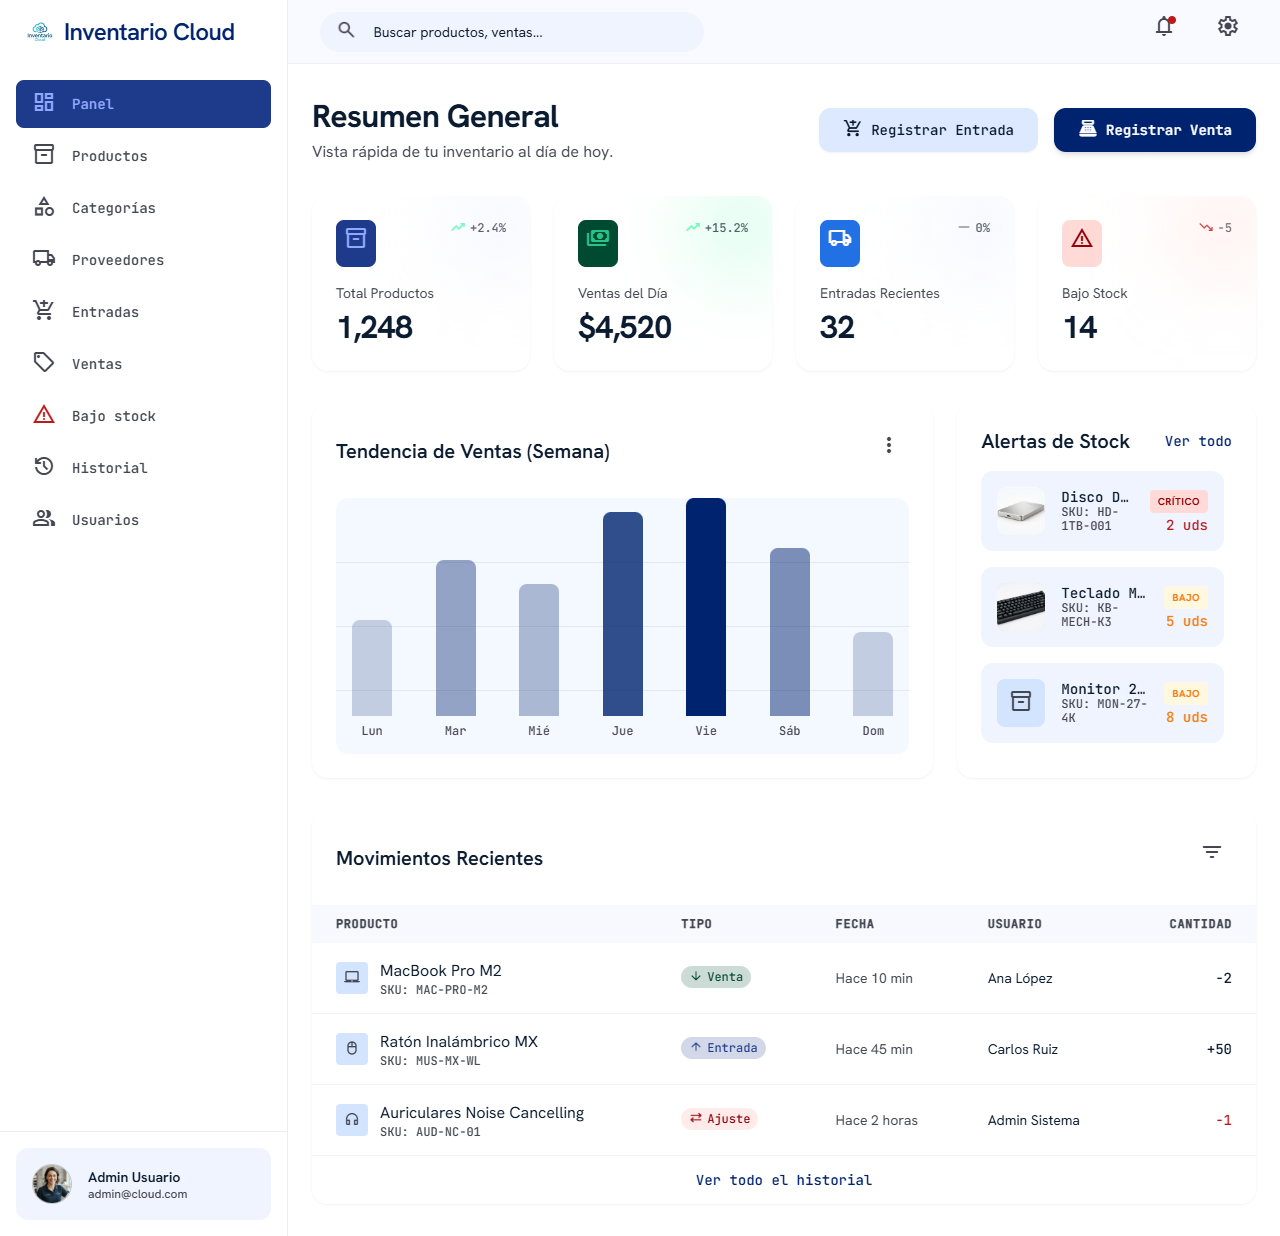
\includegraphics[height=4.2cm]{panel-escritorio.png}}{\fbox{\parbox[c][5cm][c]{0.9\linewidth}{\centering panel-escritorio.png}}}
  \par\small (a) Computadora
\end{minipage}\hspace{1cm}
\begin{minipage}[b]{0.2\textwidth}
  \centering
  \IfFileExists{venta-movil.png}{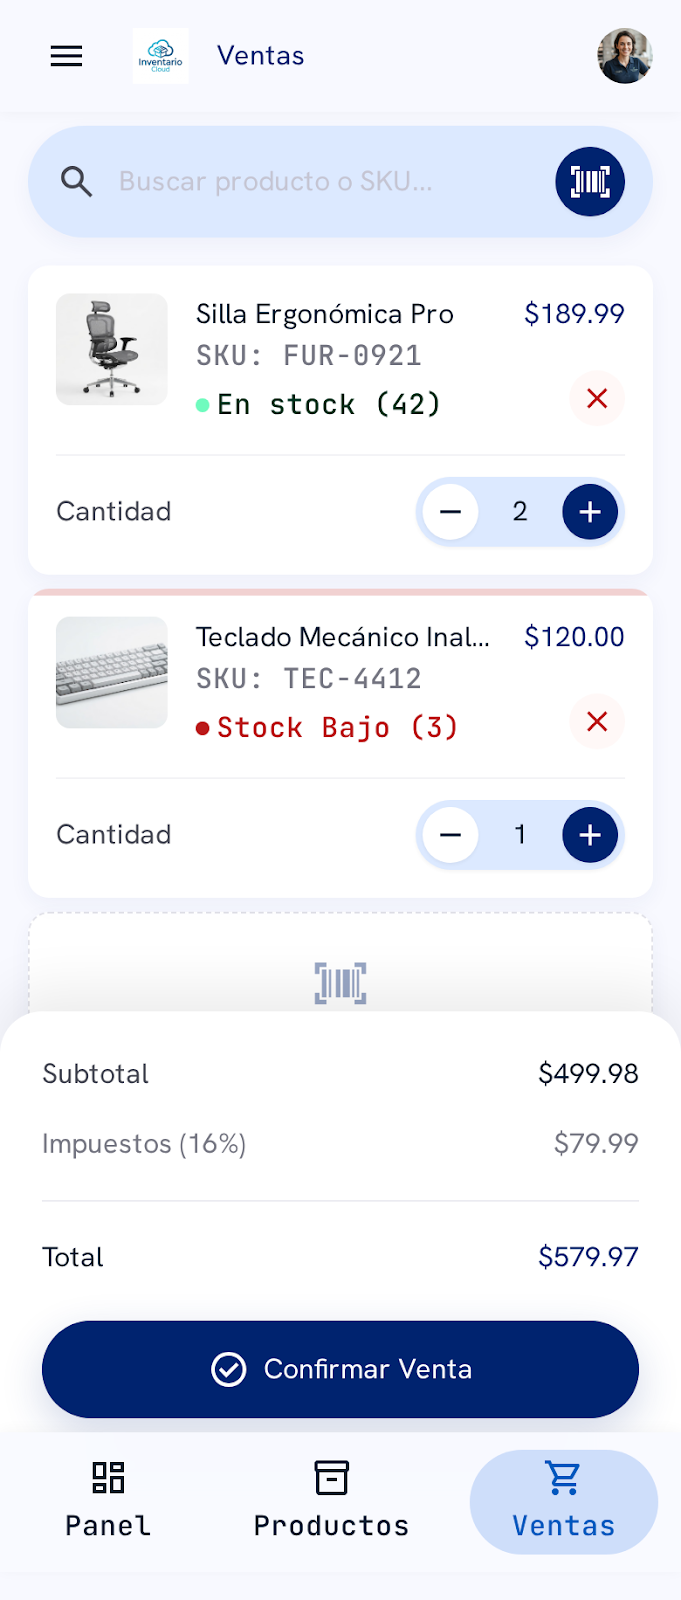
\includegraphics[height=4.2cm]{venta-movil.png}}{\fbox{\parbox[c][7cm][c]{0.9\linewidth}{\centering venta-movil.png}}}
  \par\small (b) Celular
\end{minipage}
\caption{Pantallas del sistema.}
\label{fig:prototipos}
\end{figure}

Además, para las personas que trabajan en la tienda, el sistema ofrece los servicios del cuadro~\ref{tab:funciones}.

\begin{table}[!htbp]
\centering
\footnotesize
\renewcommand{\arraystretch}{1.15}
\begin{tabularx}{\textwidth}{>{\raggedright\arraybackslash}p{3.6cm} >{\raggedright\arraybackslash}X >{\raggedright\arraybackslash}p{2.4cm}}
\toprule
\textbf{Servicio} & \textbf{Descripción} & \textbf{Quién lo usa} \\
\midrule
Inicio de sesión & Entrar y salir con correo y contraseña. Cada usuario ve solo lo que le corresponde. & Todos \\
Usuarios y roles & Cambiar el rol de un usuario y activar o desactivar cuentas. & Administrador \\
Categorías & Registrar, editar y desactivar las categorías de productos. & Administrador \\
Proveedores & Registrar y consultar los proveedores con su teléfono, correo y dirección. & Administrador \\
Productos & Registrar productos con código, precio y stock mínimo. Buscar por nombre o código. & Administrador; el empleado solo consulta \\
Entradas de mercadería & Registrar una compra a un proveedor con uno o varios productos. El stock sube solo. & Administrador \\
Ventas & Armar un carrito, confirmar la venta y descontar el stock. Si no alcanza el stock, la venta no se guarda. & Todos \\
Ajustes de stock & Corregir el stock después de un conteo físico, indicando el motivo. & Administrador \\
Alertas de bajo stock & Ver los productos que llegaron a su stock mínimo o se agotaron. & Todos \\
Historial & Ver las entradas, ventas y ajustes con fecha, usuario y cantidad. & Administrador ve todo; el empleado, lo suyo \\
Respaldo & Exportar la base de datos para no perder la información. & Administrador \\
\bottomrule
\end{tabularx}
\caption{Servicios que ofrece el sistema.}
\label{tab:funciones}
\end{table}



%=============================================================================
\begin{thebibliography}{99}
%=============================================================================
\addcontentsline{toc}{section}{Referencias}

\bibitem{flutter}
Google. (s.f.).
\newblock \emph{Flutter documentation}.
\newblock \url{https://docs.flutter.dev}

\bibitem{heizer}
Heizer, J. y Render, B. (2014).
\newblock \emph{Principios de administraci\'on de operaciones} (9.\textsuperscript{a} ed.).
\newblock Pearson Educaci\'on.

\bibitem{nist}
Mell, P. y Grance, T. (2011).
\newblock \emph{The NIST definition of cloud computing} (Special Publication 800-145).
\newblock National Institute of Standards and Technology.

\bibitem{silberschatz}
Silberschatz, A., Korth, H. F. y Sudarshan, S. (2020).
\newblock \emph{Database system concepts} (7.\textsuperscript{a} ed.).
\newblock McGraw-Hill.

\bibitem{supabasedocs}
Supabase. (s.f.).
\newblock \emph{Supabase documentation}.
\newblock \url{https://supabase.com/docs}

\end{thebibliography}

\end{document}
